%% -*- coding: utf-8; -*-

% Use 'digital' option to enable back references. This option is recommended for digital pdf version
%\documentclass[phd,american,digital]{thesispuc}%english thesis
\documentclass[mscr,american]{thesispuc}%english dissertation
%\documentclass[phd,brazilian]{thesispuc}%tese em portugês
%\documentclass[msc,brazilian]{thesispuc}%disseretação em portuguŝ


%%%
%%% Additional Packages
%%%
\usepackage{tabularx}
\usepackage{multirow}
\usepackage{multicol}
\usepackage{colortbl}
\usepackage[%
    dvipsnames,
    svgnames,
    x11names,
    fixpdftex,
    table
]{xcolor}
\usepackage{numprint}
\usepackage{textcomp}
\usepackage{booktabs}
\usepackage{amsmath}
\usepackage{enumitem}
\usepackage{amssymb}
% ABNT reference style package. The current style is the alphabetical order, if you need
% change to citation order, change in the line above 'alf' to 'num', also at the end replace
% bibliographystyle with the commented version.
\usepackage[alf,bibjustif,abnt-emphasize=bf]{abntex2cite}
%\usepackage{tikz}
%\usepackage[linesnumbered, ruled, vlined]{algorithm2e}
%\usepackage{pgfplots,pgfplotstable} 
%\usepackage{array}

%% numprint 
\npthousandsep{.}
\npdecimalsign{,}

%% ThesisPUC option
%\tablesmode{fig} %% [nada, fig, tab ou figtab]
%\algoritmsmode{none} %% [none ou use] %% Default is [use]
%\codesmode{none} %% [none ou use] %% Default is [use]
%\abreviationsmode{none} %% [none ou use] %% Default is [use]

% \makeatletter  \renewcommand\@biblabel[1]{#1}  \makeatother

%%%
%%% Counters
%%%

%% uncomment and change for other depth values
\setcounter{tocdepth}{1}
%\setcounter{lofdepth}{3}
%\setcounter{lotdepth}{3}
%\setcounter{secnumdepth}{3}

%%%
%%% Misc.
%%%

\usecolour{true}


%%%
%%% Titulos
%%%

\author{Felipe V. Côrtes}
\authorR{Cortes,Felipe} % full name

\advisor{Roberto Ierusalimschy}{Prof.} %Name LastName
\advisorR{Ierusalimschy, Roberto} %LastName, Name
% If the advisor's department is different from author's department, uncomment the next line and type the correct name and acronym of advisor's institution.
%\advisorInst{institution name}{acronym}

%\coadvisor{Otávio da Fonseca Martins Gomes}{Dr.}
%\coadvisorR{da Fonseca Martins Gomes, Otávio}
%\coadvisorInst{Centro de Tecnologia Mineral}{CETEM/MCTI}

\title{Extrator de tipos} %title in portuguese

\titleuk{Type Extractor} %title in english

%%\subtitulo{Aqui vai o subtitulo caso precise}

\day{8}
\month{March}
\year{2018}

\city{Rio de Janeiro}
\CDD{004} 
\department{Informática}
\program{Informática}
\school{Pós-Graduação em Informática}
\university{Pontifícia Universidade Católica do Rio de Janeiro}
\uni{PUC-Rio }


% %%%
% %%% Jury
% %%%

% \jury{%
%   \jurymember{Alberto Barbosa Raposo}{Prof.}
%     {Departamento de Informática}{PUC-Rio}
%   \jurymember{Waldemar Celes Filho}{Prof.}
%     {Departamento de Informática}{PUC-Rio}
% }


% %%%
% %%% Personal Resume
% %%%

% \resume{%
% % If it fit in one line use this command:
% \makebox[\textwidth][s]{Graduated in computer science by the  Harvard University.}%
% % If not just type your resume without any special command 
% }

% %%%
% %%% Acknowledgment (REMINDER TO SCHOLARSHIP STUDENTS. Do not forget to thank the agencies that supported your work.)
% %%%
% \acknowledgment{%
% \noindent To my adviser Professor Marcelo Gattass for the stimulus and partnership
% to carry out this work.
% \bigskip

% \noindent To CNPq and PUC-Rio, for the aids granted, without which this work does not
% could have been accomplished.
% \bigskip

% \noindent \textbf{For students contemplated with any CAPES scholarship, whose defense occurred as of 04 September 2018 leave the following passage:} 

% \noindent This study was financed in part by the Coordenação de Aperfeiçoamento de Pessoal
% de Nível Superior - Brasil (CAPES) - Finance Code 001.
% }


%%%
%%% Catalog prekeywords
%%%

\catalogprekeywords{%
  \catalogprekey{Informática}%
}

%%%
%%% Keywords - Don't use % at the end of /key dfinition
%%%

\keywords{%
  \key{Procesamento Geométrico}
  \key{Remoção de ruído de malha}
  \key{Vizinhança adaptativa}
}

\keywordsuk{%
  \key{Geometry Processing}
  \key{Mesh Denoising}
  \key{Adaptive Patches}
}

%%%
%%% Abstract
%%%

\abstract{%
A aquisição de malhas triangulares normalmente introduz ruídos indesejados...
}

\abstractuk{%
The acquisition of triangular meshes typically introduces undesired noise...}

%%%
%%% Dedication
%%%

\dedication{%
  To my parents, for their support\\
and encouragement.
}

%%%
%%% Epigraph
%%%

% \epigraph{%
%   My beautifull epigraph
% }
% \epigraphauthor{Wassily Kandinsky}
% \epigraphbook{Regards sur le passé}


\begin{document}
  % -*- coding: utf-8; -*-

\chapter{Introduction}
There are several reasons that motivate the adoption of statically typed languages. Maintaining large systems built with dynamic types can become a nightmare due to the lack of type information \cite{takikawa_is_2016}. Typed languages also generally has better performance because compile-time type information helps generating optimized machine code. However, programmers are frequently left empty-handed when inspecting dynamically typed code while having to re-write systems to a statically typed languaged if gradually typed languages are not an option.
\paragraph*{}
Inspired by the challenge of inspecting dynamically typed code, we built a type extractor for the Lua programming language. By inspecting a program's execution during runtime, it can generate enough information to help programmers visualize the types being transfered between functions of their program. The software output can be used as an useful documentation, while also helping programmers migrate code to a statically typed one or even for debugging.
\paragraph*{}
The document is structured as follows. In Chapter ~\ref{cha:Previous Work} we present previous work related to type systems in Lua. In Chapter ~\ref{cha:Project Scope} we describe the software goal. Chapter ~\ref{cha:Project Specification} explain the software modules and how they interact. In Chapter ~\ref{cha:Development} it's shown the software key functions, the modules relationship and basic utilization. In Chapter ~\ref{cha:Results} we present and discuss some results obtained by the type extractor on some Lua benchmarks. Finally on Chapter ~\ref{cha:Final Considerations} we present our conclusion and future work.

% \begin{figure}
% \centering
% 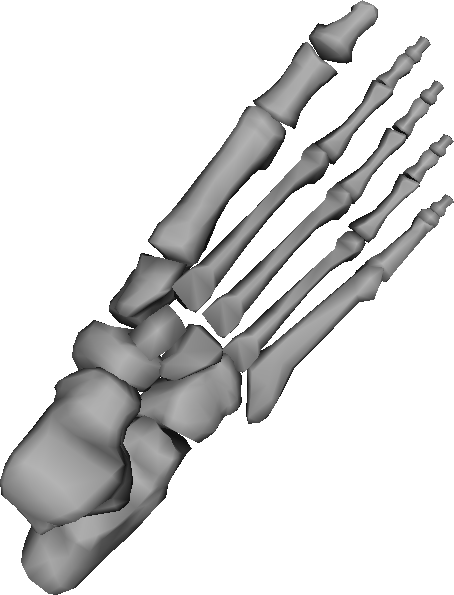
\includegraphics[width=0.45\textwidth]{pictures/image01.png}
% 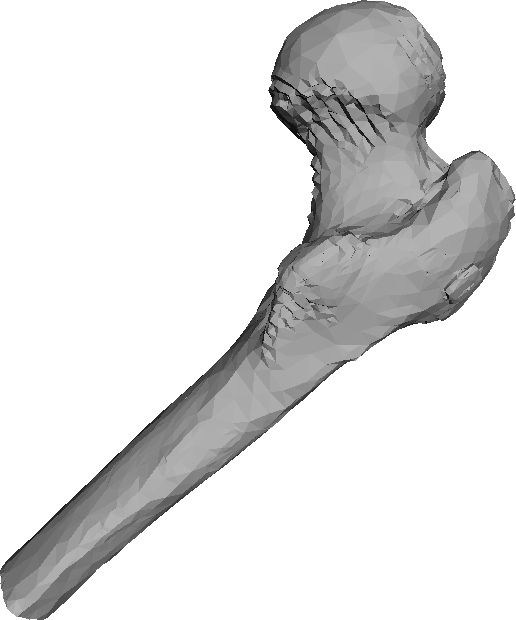
\includegraphics[width=0.45\textwidth]{pictures/image02.png}
% \caption{Meshes generated from medical data. Data obtained from the AIM$@$SHAPE Shape Repository \cite{AIMSHAPE}}
% \label{fig:example}
% \end{figure}

%This document is structured as follows. In Chapter~\ref{cha:Previous Work} we present some previous work relevant to our problem. In Chapter~\ref{cha:Proposal} we explain our proposal. In Chapter~\ref{cha:Results} we show our results. Finally, in Chapter~\ref{cha:Conclusion} we present our conclusion and future work.


 % introduction
  % -*- coding: utf-8; -*-

\chapter{Related Work}
\label{cha:Related Work}

There are 

% Early smoothing methods tried to minimize... In the figure \ref{subfig:pictures/image01.png} we see...

% \subimages{A set of three subfigures:
% (a) describes the first subfigure;
% (b) describes the second subfigure;
% (c) describes the third subfigure.}{55}
% {
%  \subimage[Bamboo-pile Vertically Inserted Position]{.45}{pictures/image01.png}
%  \subimage[Bamboo-pile Normal Inserted Position]{.45}{pictures/image02.png}\\
%  \subimage[bamboo-pile Inserted 45° angle]{.45}{example-image}
% }
% \newpage
% \csubimages{A set of six subfigures in two pages.}{55}
% {
%  \subimage[Bamboo-pile Vertically Inserted Position]{.45}{pictures/image01.png}
%  \subimage[Bamboo-pile Normal Inserted Position]{.45}{pictures/image02.png}\\
%  \subimage[bamboo-pile Inserted 45° angle]{.45}{example-image}
% }
% \ssubimages{A set of six subfigures in two pages.(Continuation)}{55}
% {
%  \subimage[Bamboo-pile Vertically Inserted Position]{.45}{pictures/image01.png}
%  \subimage[Bamboo-pile Normal Inserted Position]{.45}{pictures/image02.png}\\
%  \subimage[bamboo-pile Inserted 45° angle]{.45}{example-image}
% } % previous work
  % -*- coding: utf-8; -*-

\chapter{Project Scope}
\label{cha:Project Scope}
Type extraction for existing dymanic code is still an uncovered subject. Our software has the purpose of collecting type information from an user's program and reporting this data for documentation, inspection and code migration. The type extractor analyse each function call and return by using reflection properties of the Lua programming language. The debug library allow us to register hook functions to inspect a program's execution, computing the types present in the code.
\paragraph*{}
The type extractor can be used by two approaches, as a full program analysis or as a inspection library.
\begin{itemize}
    \item{Full Analysis:} A full program analysis is made by passing a Lua program as input to the extractor. In this approach, each possible function call and return types will be analysed.
    \item{Inspection library:} An auxiliar library, capable of registring specific functions for inspection. In this approach, the programmer can select what part of the program they want to analyse.
\end{itemize}
 These usage scenarios enables the extractor to be used as an auxiliary tool for migrating from dynamically to statically typed languages. At the end, a report containing information about parameters and return types of each analysed function is generated and shown to the user. This data serves as a good documentation for functions parameter and return types. Giving tools for understanding the type relations inside a program helps programmers to debug and optimize dynamically typed code.

%This document is structured as follows. In Chapter~\ref{cha:Previous Work} we present some previous work relevant to our problem. In Chapter~\ref{cha:Proposal} we explain our proposal. In Chapter~\ref{cha:Results} we show our results. Finally, in Chapter~\ref{cha:Conclusion} we present our conclusion and future work.



  % -*- coding: utf-8; -*-
\chapter{Project Specification}
\label{cha:Project Specification}
The objective of the type extractor is to generate a readable report for the user containing the types of parameter and return values of each function in a program's execution. With this objective in mind, we explored the reflection abilities of Lua through the following modules.
\subsection*{Type}
The Type module is responsible for categorizing Lua values into a refined type representation. As said before, our type representation is borrowed by the Pallene type system and can represent seven different categories:
\begin{flalign*}
    && \tau&:=nil \;|\; boolean \;|\; integer \;|\; float \;|\; number \;|\; string && \text{primitive types} \\
    && &| \ \left \{ \tau \right \} && \text{array type} \\
    && &| \ \left \{ l_i : \tau_i \right \} ^ {i \in 1..n} && \text{record type} \\
    && &| \ \tau_i ^ {i \in 1..n} \rightarrow \tau_j ^ {j \in 1..m}  && \text{function type} \\
    && &| \ \tau? && \text{optional type} \\
    && &| \ \{\} && \text{empty type} \\
    && &| \ any && \text{dynamic type}
\end{flalign*}
It also defines a union strategy between two types. If types are equal, then the result of a union is of the same type but if types are incopatible, a dynamic type is generated. A compatibility table is shown in~\ref{tab:comp} to help understanding this union strategy. Table~\ref{tab:res} shows the union strategy between primitive number types.
\begin{table}[!h]
    \caption{Compatibility table}
    \tiny
 \begin{tabular}{ m{1.1cm} m{0.95cm} m{0.95cm} m{0.95cm} m{0.95cm} m{0.95cm} m{0.95cm} m{0.95cm} m{0.95cm} m{0.95cm} m{0.95cm} m{0.95cm}} 

            & nil                                           & boolean                                                              & integer                                       & float                                         & number                                        & string                                        & array                                         & record                                        & empty                                         & function                                      & any                   \\ \cline{2-12} 
\multicolumn{1}{l|}{nil}      & \multicolumn{1}{l|}{\cellcolor[HTML]{036400}} & \multicolumn{1}{l|}{\cellcolor[HTML]{036400}{\color[HTML]{000000} }} & \multicolumn{1}{l|}{\cellcolor[HTML]{036400}} & \multicolumn{1}{l|}{\cellcolor[HTML]{036400}} & \multicolumn{1}{l|}{\cellcolor[HTML]{036400}} & \multicolumn{1}{l|}{\cellcolor[HTML]{036400}} & \multicolumn{1}{l|}{\cellcolor[HTML]{036400}} & \multicolumn{1}{l|}{\cellcolor[HTML]{036400}} & \multicolumn{1}{l|}{\cellcolor[HTML]{036400}} & \multicolumn{1}{l|}{\cellcolor[HTML]{036400}} & \multicolumn{1}{l|}{} \\ \cline{2-12} 
\multicolumn{1}{l|}{boolean}  & \multicolumn{1}{l|}{\cellcolor[HTML]{036400}} & \multicolumn{1}{l|}{\cellcolor[HTML]{036400}}                        & \multicolumn{1}{l|}{}                         & \multicolumn{1}{l|}{}                         & \multicolumn{1}{l|}{}                         & \multicolumn{1}{l|}{}                         & \multicolumn{1}{l|}{}                         & \multicolumn{1}{l|}{}                         & \multicolumn{1}{l|}{}                         & \multicolumn{1}{l|}{}                         & \multicolumn{1}{l|}{} \\ \cline{2-12} 
\multicolumn{1}{l|}{integer}  & \multicolumn{1}{l|}{\cellcolor[HTML]{036400}} & \multicolumn{1}{l|}{}                                                & \multicolumn{1}{l|}{\cellcolor[HTML]{036400}} & \multicolumn{1}{l|}{\cellcolor[HTML]{036400}} & \multicolumn{1}{l|}{\cellcolor[HTML]{036400}} & \multicolumn{1}{l|}{}                         & \multicolumn{1}{l|}{}                         & \multicolumn{1}{l|}{}                         & \multicolumn{1}{l|}{}                         & \multicolumn{1}{l|}{}                         & \multicolumn{1}{l|}{} \\ \cline{2-12} 
\multicolumn{1}{l|}{float}    & \multicolumn{1}{l|}{\cellcolor[HTML]{036400}} & \multicolumn{1}{l|}{}                                                & \multicolumn{1}{l|}{\cellcolor[HTML]{036400}} & \multicolumn{1}{l|}{\cellcolor[HTML]{036400}} & \multicolumn{1}{l|}{\cellcolor[HTML]{036400}} & \multicolumn{1}{l|}{}                         & \multicolumn{1}{l|}{}                         & \multicolumn{1}{l|}{}                         & \multicolumn{1}{l|}{}                         & \multicolumn{1}{l|}{}                         & \multicolumn{1}{l|}{} \\ \cline{2-12} 
\multicolumn{1}{l|}{number}   & \multicolumn{1}{l|}{\cellcolor[HTML]{036400}} & \multicolumn{1}{l|}{}                                                & \multicolumn{1}{l|}{\cellcolor[HTML]{036400}} & \multicolumn{1}{l|}{\cellcolor[HTML]{036400}} & \multicolumn{1}{l|}{\cellcolor[HTML]{036400}} & \multicolumn{1}{l|}{}                         & \multicolumn{1}{l|}{}                         & \multicolumn{1}{l|}{}                         & \multicolumn{1}{l|}{}                         & \multicolumn{1}{l|}{}                         & \multicolumn{1}{l|}{} \\ \cline{2-12} 
\multicolumn{1}{l|}{string}   & \multicolumn{1}{l|}{\cellcolor[HTML]{036400}} & \multicolumn{1}{l|}{}                                                & \multicolumn{1}{l|}{}                         & \multicolumn{1}{l|}{}                         & \multicolumn{1}{l|}{}                         & \multicolumn{1}{l|}{\cellcolor[HTML]{036400}} & \multicolumn{1}{l|}{}                         & \multicolumn{1}{l|}{}                         & \multicolumn{1}{l|}{}                         & \multicolumn{1}{l|}{}                         & \multicolumn{1}{l|}{} \\ \cline{2-12} 
\multicolumn{1}{l|}{array}    & \multicolumn{1}{l|}{\cellcolor[HTML]{036400}} & \multicolumn{1}{l|}{}                                                & \multicolumn{1}{l|}{}                         & \multicolumn{1}{l|}{}                         & \multicolumn{1}{l|}{}                         & \multicolumn{1}{l|}{}                         & \multicolumn{1}{l|}{\cellcolor[HTML]{036400}} & \multicolumn{1}{l|}{}                         & \multicolumn{1}{l|}{}                         & \multicolumn{1}{l|}{}                         & \multicolumn{1}{l|}{} \\ \cline{2-12} 
\multicolumn{1}{l|}{record}   & \multicolumn{1}{l|}{\cellcolor[HTML]{036400}} & \multicolumn{1}{l|}{}                                                & \multicolumn{1}{l|}{}                         & \multicolumn{1}{l|}{}                         & \multicolumn{1}{l|}{}                         & \multicolumn{1}{l|}{}                         & \multicolumn{1}{l|}{}                         & \multicolumn{1}{l|}{\cellcolor[HTML]{036400}} & \multicolumn{1}{l|}{}                         & \multicolumn{1}{l|}{}                         & \multicolumn{1}{l|}{} \\ \cline{2-12} 
\multicolumn{1}{l|}{empty}    & \multicolumn{1}{l|}{\cellcolor[HTML]{036400}} & \multicolumn{1}{l|}{}                                                & \multicolumn{1}{l|}{}                         & \multicolumn{1}{l|}{}                         & \multicolumn{1}{l|}{}                         & \multicolumn{1}{l|}{}                         & \multicolumn{1}{l|}{}                         & \multicolumn{1}{l|}{}                         & \multicolumn{1}{l|}{\cellcolor[HTML]{036400}} & \multicolumn{1}{l|}{}                         & \multicolumn{1}{l|}{} \\ \cline{2-12} 
\multicolumn{1}{l|}{function} & \multicolumn{1}{l|}{\cellcolor[HTML]{036400}} & \multicolumn{1}{l|}{}                                                & \multicolumn{1}{l|}{}                         & \multicolumn{1}{l|}{}                         & \multicolumn{1}{l|}{}                         & \multicolumn{1}{l|}{}                         & \multicolumn{1}{l|}{}                         & \multicolumn{1}{l|}{}                         & \multicolumn{1}{l|}{}                         & \multicolumn{1}{l|}{\cellcolor[HTML]{036400}} & \multicolumn{1}{l|}{} \\ \cline{2-12} 
\multicolumn{1}{l|}{any}      & \multicolumn{1}{l|}{}                         & \multicolumn{1}{l|}{}                                                & \multicolumn{1}{l|}{}                         & \multicolumn{1}{l|}{}                         & \multicolumn{1}{l|}{}                         & \multicolumn{1}{l|}{}                         & \multicolumn{1}{l|}{}                         & \multicolumn{1}{l|}{}                         & \multicolumn{1}{l|}{}                         & \multicolumn{1}{l|}{}                         & \multicolumn{1}{l|}{} \\ \cline{2-12} 
\end{tabular}
     \label{tab:comp}
    \end{table}
\clearpage
\begin{table}[!h]
\caption{Primitive Number Type Union}
\begin{center}
    \begin{tabular}{lll}
        type1                        & type2  & result                      \\ \hline
        \multicolumn{1}{|l}{integer} & float  & \multicolumn{1}{l|}{float} \\ \hline
        \multicolumn{1}{|l}{integer} & number & \multicolumn{1}{l|}{number} \\ \hline
        \multicolumn{1}{|l}{float}   & number & \multicolumn{1}{l|}{number} \\ \hline
        \end{tabular}
\end{center}
 \label{tab:res}
\end{table}
For recursive types, optional type and dynamic type, the following definition states the rules for union operation:
\begin{flalign*}
    && \left \{ \left. \tau_i \right \}\right. \cup \left \{ \left. \tau_j \right \}\right. &= \left \{ \left. \tau_i \cup \tau_j \right \}\right. && \text{array union} \\ \\
    && \left \{ l : \tau_i \right \} \cup \left \{ k : \tau_j \right \} &= 
    \begin{cases}
        \left \{ l_i : \tau_i \cup \tau_j \right \}& \text{ if } l = k \\ 
        \left \{ l : \tau_i \cup nil, k:\tau_j \cup nil \right \}& \text{ if } l \neq  k \\ 
       \end{cases} && \text{record union} \\ \\
    && \tau_i^{i\in 1..n} \cup  \tau_j^{j\in 1..m} &=
    \begin{cases}
     \tau_i \cup \tau_j & \text{ if } i = j \\ 
     \tau_i \cup nil & \text{ if } i > m \\ 
     \tau_j \cup nil & \text{ if } j > n
    \end{cases} && \text{function union} \\ \\ 
    && \tau \cup nil &= \tau? && \text{nil union} \\ \\
    && \tau \cup any &= any && \text{any union}
\end{flalign*}
\clearpage
\subsection*{Inspect}
The Inspect module is responsible for accessing the parameter and return values, analysing each one by our type definition. In order to access return values, the inspection module is dependent on the version 5.4 of Lua, which enables the inspection of transfered values through the debug library.

\subsection*{Hook}
A hook function is a piece of code to be executed during specific events. There are several events available to inspect but the extractor is focused on inspecting call and return events. The Hook module is resposible for configuring the inspection function to be executed at these events.

\subsection*{Report}
Generating a report consists in transforming the type information collected so far to a human readable output. The Report module is responsible for printing some function informations as well as the function types.
\\

Figure~\ref{fig:diag} shows the relationship between the project modules. Other than the modules already described here, there are modules responsible for configuring and running the extractor. Specially, the Test module validates the definitions described earlier. It asserts that the result of a type creation and type union is the one expected by an equality function between types. A type is equal to another if it has the exact same definition.

\begin{figure}
\centering
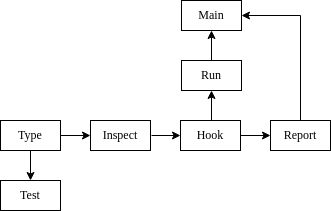
\includegraphics[width=0.45\textwidth]{pictures/module_diagram.png}
\caption{Diagram module}
\label{fig:diag}
\end{figure}






% Equation example 1:

% \begin{equation}
% \begin{split}
% \min_u \int_{x_i\in X}\int_{x_j\in X} q_{ij} u_i u_j da da + \int_{x_i\in X}||x' - x_i|| u_i da \\
% s.t. \ \ \ u\in[0,1] \ \ \land  \ \ \int_{x_i\in X}u da = a_0,
% \end{split}
% \end{equation}

% Equation exmaple 2:

% \begin{equation}
% \begin{split}
% \min_{\mathbf{u}} \alpha \mathbf{u}^T \mathbf{A}^T \mathbf{Q} \mathbf{A} \mathbf{u} +  \beta \mathbf{d}^T a' \mathbf{A} \mathbf{u} + \gamma \mathbf{u}^T \mathbf{G}^T \mathbf{G} \mathbf{u} + \delta\mathbf{f}^T a' \mathbf{A} \mathbf{u} \\
% s.t. \ \ \ \mathbf{0} \leq \mathbf{u} \leq \mathbf{1} \land \mathbf{a}^T\mathbf{u}=a_0.
% \end{split}
% \end{equation}

% Equation example 3:
% \begin{align}
% \mathbf{G}=(g_{ij}) = \left\lbrace
% \begin{array}{ll}
% \sum_{f_k\in N_f(f_i)} l_{ik} & i=j\\
% -l_{ij} & e_{ij}\in E\\
% 0 & \text{otherwise}
% \end{array}
% \right.
% \end{align}

% \lstinputlisting[label=mean,title={Mean Filter},caption={Mean Filter},language=R]{codes/mean.R}

% %% Poruguese algorithm
% %\begin{algorithm}
% %\DontPrintSemicolon
% %\Entrada{Malha e quantidade de pontos a ser amostrado}
% %\Saida{Pontos amostrados na malha}
% %\BlankLine
% %\emph{Crie um vetor de números randômicos entre $[0,1]$ com a %quantidade de pontos a ser amostrada e ordene-o}\;
% %\emph{Calcule a área total dos triângulos da malha}\;
% %\For{$i=0$ \KwTo numeroDePontos} {
% %  \emph{Navegue entre as faces acumulando a sua $\frac{area}{areaTotal}$ até achar a face com valor acumulado $\geqslant$ numerosRandomicos[i]}\;
% %  \emph{Pegue um ponto randômico dentro da face utilizando o %método de Turk e adicione no vetor do resultado}\;
% %}
% %\caption{Escolha das amostras inicias}\label{alg:sampling}
% %\end{algorithm}\DecMargin{1em}

% %% enlgish algorithm
% \begin{algorithm}
% \DontPrintSemicolon
% \KwIn{Malha e quantidade de pontos a ser amostrado}
% \KwOut{Pontos amostrados na malha}
% \BlankLine
% \emph{Crie um vetor de números randômicos entre $[0,1]$ com a quantidade de pontos a ser amostrada e ordene-o}\;
% \emph{Calcule a área total dos triângulos da malha}\;
% \For{$i=0$ \KwTo numeroDePontos} {
%   \emph{Navegue entre as faces acumulando a sua $\frac{area}{areaTotal}$ até achar a face com valor acumulado $\geqslant$ numerosRandomicos[i]}\;
%   \emph{Pegue um ponto randômico dentro da face utilizando o método de Turk e adicione no vetor do resultado}\;
% }
% \caption{Escolha das amostras inicias}\label{alg:sampling}
% \end{algorithm}\DecMargin{1em}




% \begin{flalign*}
%     && \left \{ l : \tau_i \right \} \cup \left \{ k : \tau_j \right \} = 
%     \left\{\begin{matrix}
%      \left \{ l_i : \tau_i \cup \tau_j \right \} &  \text{if} \ l = k\\ 
%      \left \{ l : \tau_i \cup nil, k:\tau_j \cup nil \right \} &  \text{if} \ l \neq  k\\ 
%     \end{matrix}\right. && \text{record union}
% \end{flalign*}
% \begin{flalign*}
%     \tau_i^{i\in 1..n} \cup  \tau_j^{j\in 1..m} = \left\{\begin{matrix}
%         \tau_i \cup \tau_j & \text{if} \ i = j\\ 
%         \tau_i \cup nil & \text{if} \ i > m\ \\
%         \tau_j \cup nil & \text{if} \ j > n\ \\
%        \end{matrix}\right. && \text{function union}
% \end{flalign*}
% \begin{flalign*}
%     \tau \cup nil = \tau? && \text{nil union}
% \end{flalign*}


%  \begin{center}
%     \( \left \{ \left. \tau_i \right \}\right. \cup \left \{ \left. \tau_j \right \}\right. = \left \{ \left. \tau_i \cup \tau_j \right \}\right. \)
% \end{center}

% \begin{center}
%     \( \left \{ l : \tau_i \right \} \cup \left \{ k : \tau_j \right \} = 
%     \left\{\begin{matrix}
%      \left \{ l_i : \tau_i \cup \tau_j \right \} &  \text{if} \ l = k\\ 
%      \left \{ l : \tau_i \cup nil, k:\tau_j \cup nil \right \} &  \text{if} \ l \neq  k\\ 
%     \end{matrix}\right. \)
% \end{center}

% \begin{center}
%     \(  \tau_i^{i\in 1..n} \cup  \tau_j^{j\in 1..m} = \left\{\begin{matrix}
%         \tau_i \cup \tau_j & \text{if} \ i = j\\ 
%         \tau_i \cup nil & \text{if} \ i > m\ \\
%         \tau_j \cup nil & \text{if} \ j > n\ \\
%        \end{matrix}\right. \)
% \end{center}
% \par
% First, the primitive types are some of the Lua basic types, added by the distinction between \textit{integer} and \textit{float}. It does not add any complexity for the types already defined by the language. The syntax of an array type is denoted by a pair of brackets with a single type. A record type is denoted by a pair of brackets with a list of labels and their respective types The \(l : \tau\) representation means that the label \textit{l} has type \(\tau\). Similarly, a function type is represented by two lists of types, where the left part represents the parameter types, while the other one represents the return types. Finally, an optional type is denoted by a type followed by a question mark.

% First, the primitive types are some of the Lua basic types, added by the distinction between \textit{integer} and \textit{float}. It does not add any complexity for the types already defined by the language:
% \begin{center}
%     \(primitive \ types\ :=\ nil \;|\; boolean \;|\; integer \;|\; float \;|\; number \;|\; string\)
% \end{center}
% The syntax of an array type is denoted by a pair of brackets with a single type:
% \begin{center}
%     \(array \ type\ :=\ \left \{ \tau \right \}\)
% \end{center}
% A record type is denoted by a pair of brackets with a list of labels and their respective types The \(l : \tau\) representation means that the label \textit{l} has type \(\tau\).
% \begin{center}
%     \(record \ type\ :=\ \left \{ l_i : \tau_i \right \} ^ {i \in 1..n} \)
% \end{center}
% Similarly, a function type is represented by two lists of types, where the left part represents the parameter types, while the other one represents the return types
% \begin{center}
%     \(function \ type\ :=\ \tau_i ^ {i \in 1..n} \rightarrow \tau_j ^ {j \in 1..m} \)
% \end{center}
% Finally, an optional type is denoted by a type followed by a question mark.
% \begin{center}
%     \(optional \ type\ :=\ \tau?\)
% \end{center}

% \begin{flalign*}
%     && \tau&:=nil \;|\; boolean \;|\; integer \;|\; float \;|\; number \;|\; string && \text{primitive types} \\
%     && &| \ \left \{ \tau \right \} && \text{array type} \\
%     && &| \ \left \{ l_i : \tau_i \right \} ^ {i \in 1..n} && \text{record type} \\
%     && &| \ \tau_i ^ {i \in 1..n} \rightarrow \tau_j ^ {j \in 1..m}  && \text{function type}
%     \end{flalign*}

% \begin{align*}
%     \tau&:=nil \;|\; boolean \;|\; integer \;|\; float \;|\; number \;|\; string \\ 
%     &| \ \left \{ \tau \right \} \\ 
%     &| \ \left \{ l_i : \tau_i \right \} ^ {i \in 1..n} \\ 
%     &| \ \tau_i ^ {i \in 1..n} \rightarrow \tau_j ^ {j \in 1..m} 
%    \end{align*}
%    \begin{align*}
%     &\qquad \textit{primitive types} \\ 
%     &\qquad  \textit{array type} \\
%     &\qquad  \textit{record type} \\
%     &\qquad  \textit{function type}
%    \end{align*}
   

%  \begin{center}
%   \begin{tabular}{l}
%     \(primitive \ types\ :=\ nil \;|\; boolean \;|\; integer \;|\; float \;|\; number \;|\; string\) \\
%     \(array \ type\ :=\ \left \{ \tau \right \}\) \\
%     \(record \ type\ :=\ \left \{ l_i : \tau_i \right \} ^ {i \in 1..n} \) \\
%     \(function \ type\ :=\ \tau_i ^ {i \in 1..n} \rightarrow \tau_j ^ {j \in 1..m} \) \\
%     \(optional \ type\ :=\ \tau?\)
%   \end{tabular}
%  \end{center}
%  Primitive types are some of Lua basic types, added by the distinction between \textit{integer} and \textit{float}. The array, record and function types are recursive definitions, it means that the symbol \(\tau\) can represent any of the type definitions. The syntax of an array type is denoted by a pair of brackets with a single type. A record type is denoted by a pair of brackets with a list of labels and their respective types The \(l : \tau\) representation means that the label \textit{l} has type \(\tau\). Similarly, a function type is represented by two lists of types, where the left part represents the parameter types, while the other one represents the return types. At last, an optional type is denoted by the type definition followed by a question mark.
 
% \begin{flalign*}
%     && \left \{ \left. \tau_i \right \}\right. \cup \left \{ \left. \tau_j \right \}\right. = \left \{ \left. \tau_i \cup \tau_j \right \}\right. && \text{array union} \\ \\
%     && \left \{ l : \tau_i \right \} \cup \left \{ k : \tau_j \right \} = 
%     \left\{\begin{matrix}
%      \left \{ l_i : \tau_i \cup \tau_j \right \} &  \text{if} \ l = k\\ 
%      \left \{ l : \tau_i \cup nil, k:\tau_j \cup nil \right \} &  \text{if} \ l \neq  k\\ 
%     \end{matrix}\right. && \text{record union} \\ \\
%     && \tau_i^{i\in 1..n} \cup  \tau_j^{j\in 1..m} = \left\{\begin{matrix}
%         \tau_i \cup \tau_j & \text{if} \ i = j\\ 
%         \tau_i \cup nil & \text{if} \ i > m\ \\
%         \tau_j \cup nil & \text{if} \ j > n\ \\
%        \end{matrix}\right. && \text{funciton union} \\ \\
%     && \tau \cup nil = \tau? && \text{nil union} \\ \\ 
%     && integer \cup float = number && \text{nil union}
% \end{flalign*}



  % -*- coding: utf-8; -*-

\chapter{Development}
\label{cha:Development}

Table example. Table~\ref{tab:res} shows results. 

\begin{table}[!h]
\caption{Results for devil mesh}
\tiny
\begin{center}
\begin{tabular}{ m{1.1cm} m{0.95cm} m{0.95cm} m{0.95cm} m{0.95cm} m{0.95cm} m{0.95cm} m{0.95cm} m{0.95cm} m{0.95cm} } 
 & Mean Vertex Distance & L2 Vertex Based & Mean Quadric & MSAE & L2 Normal Based & Tangential & Mean Discrete Curvature & Area Error & Volume Error\\ 
 \hline 
\cite{FDC03} & 0.061277 & 0.110973 & 0.236219 & 19.697900 & 0.055170 & 0.047678 & 0.090284 & 0.051443 & 0.045645 \\ 
 \cite{JDD03} & 0.001293 & 0.002800 & 0.002289 & 21.237300 & 0.021589 & 0.013026 & 0.087991 & 0.000364 & 0.002621 \\ 
 \cite{SRML07} & 0.001439 & 0.002880 & 0.003540 & 14.043200 & 0.012654 & 0.008911 & 0.055849 & 0.007806 & 0.000582 \\ 
 \cite{ZFAT11} & \cellcolor{blue!25}0.000713 & \cellcolor{blue!25}0.001537 & 0.001824 & 12.171400 & \cellcolor{blue!25}0.009654 & \cellcolor{blue!25}0.005781 & \cellcolor{blue!25}0.054567 & 0.005617 & \cellcolor{blue!25}0.000425 \\ 
 \cite{HS13} & 0.002531 & 0.004560 & 0.007108 & 13.830100 & 0.017459 & 0.010314 & 0.114528 & 0.001686 & 0.001786 \\ 
 \cite{ZDZBL15} & 0.001623 & 0.003079 & 0.005048 & \cellcolor{blue!25}10.454200 & 0.015233 & 0.008054 & 0.094668 & 0.002629 & 0.001326 \\ 
 \cite{YRP16} & 0.000737 & 0.001548 & \cellcolor{blue!25}0.001493 & 16.880800 & 0.014129 & 0.006974 & 0.079952 & \cellcolor{blue!25}0.000209 & 0.002375 \\ 
 Ours & 0.000987 & 0.001902 & 0.002686 & 11.574200 & 0.010632 & 0.006796 & 0.075106 & 0.003970 & 0.000722 \\ 
 \end{tabular}
\end{center}
 \label{tab:res}
\end{table}

\section{Comparison}
  \chapter{Results}
\label{cha:Results}
In this section, we will give some examples of generated reports obtained by passing a full program as input to the type extractor. The program analysis is not supposed to be fast. The overhead of a Lua call for each hook is high enough to leverage time performance. In this section we will present some reports generated by the extractor when analysing simple Lua programs and also Lua benchmark programs.

\section*{Basic}
A basic result of the extractor is represented by the Image~\ref{fig:basic1}. The output generated is related to the execution of Code~\ref{basic1}. Image~\ref{fig:basic2} shows the output for Code~\ref{basic2}. In this example, regardless of the input type, because the result generated by \textit{type} is always an string.
\lstinputlisting[label=basic1,title={Basic example 1},caption={Basic example 1}, language={[5.0]Lua}]{codes/basic_1.lua}
\lstinputlisting[label=basic2,title={Basic example 2},caption={Basic example 2}, language={[5.0]Lua}]{codes/basic_2.lua}
\begin{figure}
    \centering
    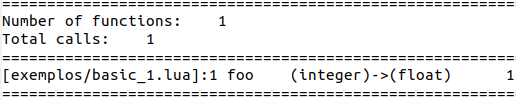
\includegraphics[width=0.65\textwidth]{pictures/basic1.png}
    \caption{Basic example 1}
    \label{fig:basic1}
\end{figure}
\begin{figure}
    \centering
    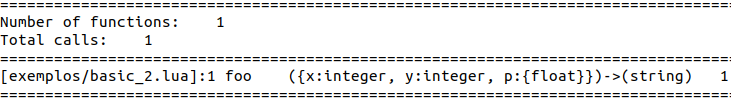
\includegraphics[width=0.85\textwidth]{pictures/basic2.png}
    \caption{Basic example 2}
    \label{fig:basic2}
\end{figure}
Another useful example is shown by the output of Code~\ref{basic3} and its output in Image~\ref{fig:basic3}. Instead of analysing transfered values only in the return event, the extractor analyses the parameter type in a call event, before any other assignment is made, preserving the type of the variables before the function's execution.
\lstinputlisting[label=basic3,title={Basic example 3},caption={Basic example 3}, language={[5.0]Lua}]{codes/basic_3.lua}
\begin{figure}
    \centering
    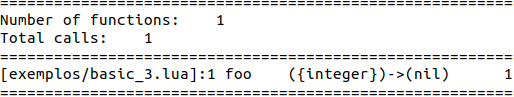
\includegraphics[width=0.85\textwidth]{pictures/basic3.png}
    \caption{Basic example 3}
    \label{fig:basic3}
\end{figure}
Image~\ref{fig:basic4} exeplifies a union of function types, generated by the execution of Code~\ref{basic4}. An union between an array of integer and a boolean type results in a dynamic type.
\lstinputlisting[label=basic4,title={Basic example 4},caption={Basic example 4}, language={[5.0]Lua}]{codes/basic_4.lua}
\begin{figure}
    \centering
    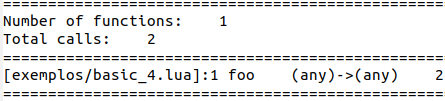
\includegraphics[width=0.85\textwidth]{pictures/basic4.png}
    \caption{Basic example 4}
    \label{fig:basic4}
\end{figure}
Finally, Image~\ref{fig:basic5} shows the handling of proper tail calls in action. Code~\ref{basic5} has two functions, where the last statement of \textit{foo} is a call to \textit{boo}, when the return event of this function is triggered, the return type of the calling function is updated correctly.
\clearpage
\lstinputlisting[label=basic5,title={Basic example 5},caption={Basic example 5}, language={[5.0]Lua}]{codes/basic_5.lua}
\begin{figure}
    \centering
    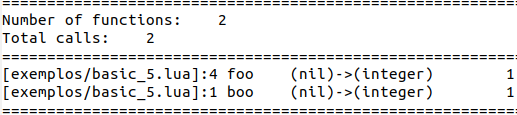
\includegraphics[width=0.85\textwidth]{pictures/basic5.png}
    \caption{Basic example 5}
    \label{fig:basic5}
\end{figure}









% \lstinputlisting[label=mean2,title={Mean Filter},caption={Mean Filter},language=R]{codes/mean.R}
  \chapter{Final Considerations}
\label{cha:Final Considerations}

We proposed an algorithm for triangular mesh denoising with detail preservation...

\lstinputlisting[label=mean2,title={Mean Filter},caption={Mean Filter},language=R]{codes/mean.R}
  %% ...
  \arial
  \bibliographystyle{abnt-alf} % \bibliographystyle{abnt-num}
  \bibliography{srs} 
\end{document}
